\documentclass[10pt]{article}
\usepackage{labreport}
\begin{document}
\PageTitle{01 / EXECUTIVE SUMMARY}{Studio North: is growth\newline becoming more valuable?}{Customer acquisition, monthly renewal and contribution economics | 24 monthly acquisition cohorts, 2024-01 through 2025-12; data cutoff 2026-01-01}
\Section{The business and the decision}
Studio North sells a monthly creative-work membership to independent professionals. Standard and premium plans combine ready-to-use templates with guided learning; members can also purchase workshops and other add-ons. Each month, members choose whether to renew. Search campaigns and partner workshops bring customers with two stated priorities: save time or build skills.

Management needs to know whether successive acquisition cohorts create more durable contribution, at a cost the company can recover quickly enough to fund growth. Company scale, customer quality and marketing incrementality answer different parts of that decision.
\Takeaway{The matched-age endpoints show lower blended CAC, higher contribution and stronger cash recovery. Renewal is not clearly improving across successive cohorts; short campaign tests do not yet establish a profitable acquisition expansion.}
\Metric{ACQUISITION EFFICIENCY}{\$106 $\rightarrow$ \$73}{blended CAC per acquired customer}\hfill
\Metric{CUSTOMER VALUE}{\$123 $\rightarrow$ \$144}{six-month contribution per customer}\hfill
\Metric{CASH RECOVERY}{\$18 $\rightarrow$ \$71}{six-month cash after blended CAC}
\Evidence{Matched-age comparison: 2024-01 to 2025-07. Values above are rounded to dollars; the evidence table reports cents.}
\Section{What the evidence establishes}
\par\begin{tabularx}{\linewidth}{@{}YYYY@{}}\toprule
\textbf{Evidence} & \textbf{Earlier} & \textbf{Later} & \textbf{Interpretation}\\\midrule
Sixth-month retained share & 63.1\% & 67.9\% & Observed at age index 5\\
Blended CAC & \$105.79 & \$72.99 & Tracked spending / all acquired people\\
Six-month contribution / customer & \$123.39 & \$144.05 & Cumulative, after variable costs\\
Six-month cash after acquisition & \$17.60 & \$71.06 & Per original acquired customer\\
Joining cohort & 2024-01 & 2025-07 & Latest cohort with six observed ages\\
\bottomrule\end{tabularx}\par
\Section{Recommended management response}
\textbf{Action.} Marketing and Analytics should preserve controls and extend both campaign follow-ups through the cash-recovery horizon. Finance should monitor six-month cash against the trailing six mature cohorts' median of \$50.36 per customer, not use it as an automatic causal gate. Product should investigate the Search / save-time renewal weakness before assuming conversion gains imply durable value.
Incremental contribution after media per assigned prospect: search / save time: \$1.16 over 31 days (95\% interval \$-0.62 to \$2.94); partner / build skill: \$-0.36 over 30 days (95\% interval \$-2.26 to \$1.54). 2 of 2 intervals include zero; neither the sign nor the ranking of point estimates warrants a scale-or-stop decision.
\Section{What would change the decision}
For immature cohorts, value depends on future renewals and spending. Treat their LTV as a conditional forecast. Scale a campaign only when a randomized comparison supports incremental contribution over a relevant window; historical attributed CAC alone cannot establish that return. Retain the cost and cash-recovery constraints when a campaign produces more revenue.
\Boundary{All customer records describe an illustrative business and are synthetic. The analysis covers recorded variable costs and acquisition spending, not fixed operating costs, financing or taxes. It therefore does not establish company profitability.}
\Evidence{The management pages summarize the diagnosis and action. Appendices document the model, parameter estimates, validation, data architecture and dataset-level Universal Customer View.}

\NewPage
\PageTitle{02 / OBSERVED COHORT ECONOMICS}{Compare customer quality\newline at a common age}{A joining cohort contains customers whose first successful payment occurred in the same month. Future ages remain unobserved.}
\FullFig{cohort-triangles.pdf}{3.25in}
\Evidence{Saved SQL outputs: \texttt{cohort\_totals.csv} and \texttt{cohort\_cash\_economics.csv}. Age 0 is the first paid month. Cash balance is cumulative contribution less tracked acquisition spending, divided by original cohort size. These six cohorts are an evenly spaced subset of the sorted 24-cohort sequence, including its endpoints; they were not selected for favorable results.}
\Section{Acquisition efficiency and durability must move together}
At the common sixth age month, retained share is higher: 63.1\% for 2024-01 versus 67.9\% for 2025-07. Blended CAC is lower: \$105.79 versus \$72.99. It divides tracked spending by all acquired people; organic control buyers enter that denominator in cohorts where they occur. Paid-source CAC has a different denominator. These are descriptive comparisons, not campaign effects. At the same age, cumulative contribution per acquired customer changes from \$123.39 to \$144.05; cash after acquisition changes from \$17.60 to \$71.06. Both calculations use recorded variable costs.
\FullFig{retention-and-revenue.pdf}{2.05in}
\Evidence{Retained share uses original cohort membership; revenue retention uses each cohort's first-period revenue. Revenue can change because of the number of renewing members, their plan mix or add-on spending. Product activity is not a substitute for a renewal record.}
\Takeaway{The trajectory matters as well as the cutoff. A stronger first month does not establish longer customer life, while a customer-count decline can coexist with more spending by the members who remain.}

\NewPage
\PageTitle{03 / CUSTOMER GROUPS}{Check whether progress\newline survives the customer mix}{Observed renewal trajectories by acquisition channel and stated need; each panel uses the same axes.}
\FullFig{channel-segment-retention.pdf}{3.7in}
\Evidence{Saved SQL output: \texttt{cohort\_age\_summary.csv}. Curves divide retained members by the original cohort--channel--need cell. No missing future observations are filled with zeros.}
\Section{Within-group diagnosis}
The two displayed endpoints improve in 3 of 4 channel-by-need cells, but the intervening curves do not establish a steady renewal trend. Search / save time changes from 63\% to 61\% retained at age 5. Its short-window experimental conversion response does not establish better subsequent renewal.
\Section{A useful segmentation separates relevant differences}
The primary need grouping has the lowest within-group variance in six-month contribution (4,414.7 dollars squared), but the reduction versus the next-best scheme is 2.3\%. This is a modest separation, with substantial residual customer heterogeneity. Use the groups to organize the diagnosis; a need label does not make their economics homogeneous.
\par\begin{tabularx}{\linewidth}{@{}YYYY@{}}\toprule
\textbf{Grouping} & \textbf{Variance (dollars squared)} & \textbf{Groups} & \textbf{Smallest group}\\\midrule
age band & 4,520.2 & 2 & 1718\\
primary need & 4,414.7 & 2 & 1578\\
region & 4,520.3 & 2 & 1725\\
\bottomrule\end{tabularx}\par
\Evidence{Comparison uses the same mature-customer sample and the same six-month outcome. Smaller within-group variance means more homogeneous observed outcomes within the chosen groups; it does not imply identical customers or establish a causal effect of a need or channel.}
\Boundary{Stated need is known before acquisition. It can support targeting and journey interpretation. Joining month defines a cohort, not a segment. Survey evaluations and observed behavior can suggest explanations to test, but neither proves why a customer renewed or left.}

\NewPage
\PageTitle{04 / COMPANY ECONOMICS}{Retained cohorts determine\newline how growth accumulates}{The company is the sum of its acquisition cohorts at different ages, not the latest cohort scaled up.}
\FullFig{company-cohort-layers.pdf}{3.15in}
\Evidence{Saved SQL output: \texttt{company\_month.csv}. Each layer is a joining cohort's active customers at the displayed calendar month. Layer totals are reconciled to independently saved company totals before plotting.}
\FullFig{company-economics.pdf}{1.75in}
\Section{Scale and cash recovery are separate tests}
New acquisition adds customers immediately. Renewals preserve older layers and their contribution, reducing the replacement acquisition required to sustain scale. The lower chart compares recorded contribution with acquisition spending in each calendar month; it is not cumulative retained customers or a profit statement.
In 2025-12, recorded contribution was \$84,335 and acquisition spending was \$16,529, leaving \$67,806 before fixed costs, financing and taxes. This period result should be read alongside the age-aligned cohort comparison, rather than used as a substitute for it.
\Section{Operating implication}
Track both the common-age economics of each joining cohort and the company's accumulated contribution. A favorable acquisition metric can coexist with slower cash recovery when renewals weaken. A growing customer base can also conceal deterioration if management replaces departing customers with increasingly costly new ones.
\Boundary{Cash payback is undiscounted: the first age at which cumulative contribution covers the acquisition investment. The LTV calculation that follows discounts expected monthly contribution and uses a common, explicit horizon.}

\NewPage
\PageTitle{05 / MODEL AND VALUE FORECAST}{Forecast monthly renewal\newline before forecasting value}{Hierarchical shifted-Beta-Geometric retention + Gamma gross revenue; NumPyro NUTS}
\Section{How the model represents the business}
Each member has a persistent churn propensity. Within a cohort/need/channel cell, propensities follow one Beta distribution. After t-1 renewals, churn hazard is $\alpha/(\alpha+\beta+t-1)$; observed survivors follow a Binomial with the previous survivor count as its risk set. Mean propensity varies with need, channel, cohort trend and a partially pooled cohort effect. Concentration varies with need and channel. Variance is $\mu(1-\mu)/(\phi+1)$. Falling aggregate churn can reflect survivor selection, not improvement in each individual's loyalty. Pending renewals and future ages are unobserved, not failures. Age zero establishes acquisition and supplies no renewal trial. Churn is absorbing in this business.
\[\operatorname{net\,LTV}_{H}=\sum_{a=0}^{H-1}\frac{\operatorname{E}[\text{contribution}_{a}\mid\text{observed history}]}{(1+d)^{a+1}}-\operatorname{CAC}.\]
\Evidence{Gross payment revenue follows a Gamma distribution with shape proportional to observed retained members. Expected revenue per retained member varies with log age, cohort trend, need and channel. Observed age-aligned net and contribution shares translate future gross revenue into economics. Keep observed revenue and contribution; forecast recursively from the last observed survivors. All cohorts are valued over the same 12 monthly receipts, discounting at 1\% per month. Forecast bands and the probability of nonnegative expected cash cover parameter uncertainty, not renewal/revenue process noise or all future business risk. The main retention model extends Fader--Hardie's shifted-Beta-Geometric approach; the revenue model adapts Orduz's Gamma structure. An Orduz-inspired neural retention model is a separate validation benchmark, not the source of executive LTV. Parameter estimates and held-out checks appear in the appendix.}
\FullFig{ltv-and-cac.pdf}{2.5in}
\Evidence{Posterior parameter uncertainty conditional on the single-Beta model and fixed future economics; not a full predictive interval. The lower strip shows the forecast share of common 12-month LTV. Dotted markers identify experiment months with organic control buyers in the denominator. Blended CAC divides tracked spending by all acquired customers; it is not the causal cost of the next customer.}
\Section{Management interpretation}
Across the cohort sequence, common-horizon contribution LTV combines observed receipts with a growing predicted remainder; the strip makes that dependence visible. Net of blended CAC, the endpoint comparison is \$104.90 for 2024-01 versus \$163.21 for 2025-12. This is not a monotonic improvement claim. The newest value is 89\% forecast, with a 5th--95th parameter range of \$150.96 to \$175.83.
\Boundary{Future net revenue and contribution shares of payment revenue use observed channel-by-need-by-age shares, with the same group's observed renewal ages (age>=1) as fallback. Shares are fixed assumptions, not causally identified or assigned posterior uncertainty. Predicted customer value is not experimentally identified campaign return. A favorable average LTV-to-CAC comparison still requires a cash-recovery constraint and evidence that the next acquisition investment creates additional value.}

\NewPage
\PageTitle{06 / CAMPAIGNS AND ACTION}{Require the next campaign\newline to beat its own baseline}{Randomized assignment includes all eligible prospects, including those who never purchase. Each test keeps its own control and follow-up window.}
{\fontsize{8}{10}\selectfont \par\begin{tabularx}{\linewidth}{@{}p{.25\linewidth}lrrrr@{}}\toprule
\textbf{Test} & \textbf{Arm} & \textbf{Assigned} & \textbf{Buyers} & \textbf{Contribution} & \textbf{Media}\\\midrule
search / save time & control & 250 & 30 & \$739.00 & \$0.00\\
search / save time & treatment & 250 & 70 & \$1,679.25 & \$650.00\\
partner / build skill & control & 250 & 34 & \$834.85 & \$0.00\\
partner / build skill & treatment & 250 & 62 & \$1,644.55 & \$900.00\\
\bottomrule\end{tabularx}\par}
\FullFig{experiment-effects.pdf}{2.1in}
\Evidence{Saved SQL outputs: \texttt{experiment\_summary.csv} and \texttt{experiment\_effects.csv}. Whiskers are approximate 95\% intervals from all-assigned contribution variances, including nonbuyer zeros. Fixed media costs shift the mean, not its sampling variance. These 30/31-day windows are shorter than the cohorts' cash-recovery horizon; they do not measure lifetime campaign return.}
\Section{The same economics apply to treatment and control}
For each arm, net revenue less recorded variable costs gives contribution. Compare contribution per assigned eligible prospect, then subtract the treatment's additional media cost. Control purchases remain in the baseline rather than receiving campaign credit.
\[
\Delta\text{contribution after media per prospect}
=\frac{C_T-M_T}{N_T}-\frac{C_C-M_C}{N_C}.
\]
\Section{Management actions and accountability}
\par\begin{tabularx}{\linewidth}{@{}p{.18\linewidth}YY@{}}\toprule
\textbf{Accountable team} & \textbf{Next action} & \textbf{Decision evidence}\\\midrule
Marketing + Finance & Defer expansion or rejection based only on the short-window profit estimates; monitor recovery against mature-cohort experience. & Age-aligned value and cash, alongside uncertainty in incremental returns.\\
Product + Operations & Investigate Search / save-time renewal weakness despite its positive short-term conversion response. & Renewal events, product actions and expressed customer evaluations.\\
Marketing + Analytics & Preserve both controls and extend follow-up through the acquisition cash-recovery horizon. & Contribution after media per assigned prospect, including nonbuyers, with uncertainty.\\
Data + Analytics & Refresh the evidence from the source exports and review forecast misses before releasing the decision report. & SQL reconciliation, model holdouts, parameter output and file hashes.\\
\bottomrule\end{tabularx}\par
\Boundary{Do not multiply experimental conversion lift by the predicted LTV of observed buyers and label the product an established lifetime campaign effect. The tested population, outcome window and valuation assumptions must remain visible.}

\NewPage
\PageTitle{A1 / MODEL SPECIFICATION}{Parameter meanings\newline and fitted estimates}{Technical appendix | The inference model is distinct from the process used to generate the synthetic customer records.}
\Section{Likelihood, heterogeneity and economic conversion}
Each member has a persistent churn propensity. Within a cohort/need/channel cell, propensities follow one Beta distribution. After t-1 renewals, churn hazard is $\alpha/(\alpha+\beta+t-1)$; observed survivors follow a Binomial with the previous survivor count as its risk set. Mean propensity varies with need, channel, cohort trend and a partially pooled cohort effect. Concentration varies with need and channel. Variance is $\mu(1-\mu)/(\phi+1)$. Falling aggregate churn can reflect survivor selection, not improvement in each individual's loyalty. Gross payment revenue follows a Gamma distribution with shape proportional to observed retained members. Expected revenue per retained member varies with log age, cohort trend, need and channel. Observed age-aligned net and contribution shares translate future gross revenue into economics. Pending renewals and future ages are unobserved, not failures. Age zero establishes acquisition and supplies no renewal trial. Churn is absorbing in this business.
\[\begin{aligned}p_{i,g}&\sim\operatorname{Beta}(\alpha_g,\beta_g), & \alpha_g&=\mu_g\phi_g, &\beta_g&=(1-\mu_g)\phi_g,\\N_{g,t}\mid N_{g,t-1}&\sim\operatorname{Binomial}(N_{g,t-1},1-h_g(t)), & h_g(t)&=\frac{\alpha_g}{\alpha_g+\beta_g+t-1}.\end{aligned}\]
\Evidence{$g$ indexes a cohort--need--channel cell; $t=1$ is its first renewal. Mean-churn coefficients use a logit link; concentration and revenue use log links. Search and save-time customers are the reference groups. Retention cohort trend is $(\text{index}-11.5)/11.5$; revenue cohort trend is $(\text{index}-11.5)/12$. Revenue log-age is $\log(1+\text{age})$. Cohort index runs from 0 to 23.}
{\fontsize{7.8}{9.5}\selectfont \par\begin{tabularx}{\linewidth}{@{}p{.22\linewidth}p{.20\linewidth}rrYr@{}}\toprule
\textbf{Parameter} & \textbf{Prior} & \textbf{Mean} & \textbf{5th--95th} & \textbf{R-hat} & \textbf{ESS}\\\midrule
cohort\_scale & HalfNormal(0.25) & 0.055 & 0.006 to 0.115 & 1.001 & 1,412\\
concentration\_beta[intercept] & Normal(log(4),1) & 1.450 & 1.249 to 1.659 & 1.000 & 2,556\\
concentration\_beta[build\_skill] & Normal(0,0.5) & 0.232 & -0.038 to 0.505 & 1.001 & 3,170\\
concentration\_beta[partner] & Normal(0,0.5) & 0.042 & -0.227 to 0.319 & 1.000 & 2,896\\
concentration\_beta[organic] & Normal(0,0.5) & -0.087 & -0.832 to 0.655 & 1.000 & 5,560\\
mean\_beta[intercept] & Normal(-2.5,1) & -1.818 & -1.916 to -1.718 & 1.000 & 2,369\\
mean\_beta[build\_skill] & Normal(0,0.5) & -0.307 & -0.429 to -0.185 & 1.001 & 3,381\\
mean\_beta[partner] & Normal(0,0.5) & -0.076 & -0.195 to 0.043 & 1.000 & 2,791\\
mean\_beta[organic] & Normal(0,0.5) & 0.078 & -0.309 to 0.452 & 1.000 & 5,229\\
mean\_beta[cohort\_trend] & Normal(0,0.5) & -0.025 & -0.110 to 0.059 & 1.000 & 4,770\\
revenue\_beta[intercept] & Normal(-0.5,0.8) & -0.601 & -0.606 to -0.596 & 1.000 & 6,944\\
revenue\_beta[log1p\_age] & Normal(0.1,0.8) & 0.106 & 0.104 to 0.109 & 0.999 & 5,974\\
revenue\_beta[cohort\_trend] & Normal(0,0.8) & 0.021 & 0.017 to 0.026 & 0.999 & 7,944\\
revenue\_beta[build\_skill] & Normal(0,0.8) & 0.056 & 0.052 to 0.060 & 1.000 & 8,898\\
revenue\_beta[partner] & Normal(0,0.8) & -0.002 & -0.006 to 0.003 & 0.999 & 7,312\\
revenue\_beta[organic] & Normal(0,0.8) & -0.019 & -0.043 to 0.005 & 0.999 & 6,587\\
revenue\_shape & LogNormal(log(4),0.8) & 17.309 & 16.192 to 18.469 & 0.999 & 7,994\\
\bottomrule\end{tabularx}\par}
\Evidence{The 24 standardized cohort offsets z have posterior means from -0.691 to 0.769; multiply each draw by cohort\_scale to obtain its log-odds shift. Their largest R-hat is 1.001; smallest effective sample size is 4,250. The complete parameter\_summary.csv provides every cohort effect, prior, interval and interpretation.}
\Evidence{At the coefficient means, Search / save time at centered cohort trend and zero offset has mean latent monthly churn mu=14.0\% and concentration phi=4.26. The cohort-trend coefficient's 5th--95th interval is -0.110 to 0.059; it includes zero and does not establish a renewal improvement trend.}
\Evidence{Posterior means and 5th--95th percentiles are read from the saved, hash-bound parameter output. Units and reference groups are stated with the parameter definitions; transformed parameters are not interchangeable with their latent log-scale values.}
\Section{Estimation and reproducibility}
\par\begin{tabularx}{\linewidth}{@{}p{.36\linewidth}Y@{}}\toprule
\textbf{Setting or diagnostic} & \textbf{Recorded value}\\\midrule
Inference & NUTS\\
Chains / warmup / samples & 4 / 1000 / 1000 per chain\\
Posterior forecast draws & 400\\
Maximum R-hat / minimum ESS & 1.001 / 1,412\\
Divergences & 0\\
Seed / numerical backend & 20261116 / cpu / float64\\
\bottomrule\end{tabularx}\par

\NewPage
\PageTitle{A2 / RETENTION FORECASTS}{Show the unobserved\newline renewal path explicitly}{Technical appendix | The same model forecasts retained customers, then converts that path into revenue and contribution.}
\FullFig{retention-forecast.pdf}{3.25in}
\Evidence{Saved model output: \texttt{forecast\_curve.csv}. Each panel uses its original acquired-customer denominator. Solid points are observed; dashed lines are forecast expected retention; shading is the 5th--95th posterior parameter range. The vertical marker is the observation boundary.}
\Section{The amount of observed renewal history matters}
The complete cohort supplies an observed reference. The intermediate cohort has some renewal history but still requires extrapolation. The newest cohort has only its acquisition month: it has \textbf{zero observed renewal decisions}. Its future path borrows information from older cohorts, stated needs, acquisition channels and the model's partially pooled cohort distribution.
\FullFig{forecast-detail.pdf}{1.65in}
\Evidence{Observed contribution is retained; only the unobserved remainder is predicted. The newest cohort's forecast relies on older cohorts until its own renewal history becomes available.}
\Boundary{These are expected customer paths conditional on fitted parameters. The bands exclude future customer-level Bernoulli variation, uncertain economic conversion and changes in the business regime. A narrow parameter band is not evidence that those risks are small.}

\NewPage
\PageTitle{A3 / VALIDATION}{Separate fitted agreement\newline from prediction performance}{Technical appendix | A model can describe observed counts closely and still miss the future.}
\FullFig{recent-cohort-fit-check.pdf}{2.9in}
\Evidence{Saved SQL/model output: \texttt{model\_fit\_checks.csv}. These are in-sample, one-step fitted residuals conditional on previous observed customer counts. They are not held-out forecast errors.}
\Section{Held-out performance}
\Evidence{Training includes 2025-09; withheld months are 2025-10, 2025-11, 2025-12.}
Withheld cells: 258. Retained-count mean absolute error: 1.11. Revenue weighted absolute percentage error: 6.1\%. A separate training-only forecast checks complete 12-month values: LTV mean absolute error \$3.13 versus \$25.21 for its baseline. These tests evaluate prediction, not campaign effects.
\par\begin{tabularx}{\linewidth}{@{}p{.28\linewidth}rrY@{}}\toprule
\textbf{Measure} & \textbf{Model} & \textbf{Baseline} & \textbf{Interpretation}\\\midrule
Retained-count MAE & 1.11 & 1.89 & People per withheld cell\\
Retained-count WAPE & 4.7\% & Not reported & Retained customers, not revenue\\
Revenue WAPE & 6.1\% & 10.8\% & Withheld calendar months\\
12-month LTV MAE & \$3.13 & \$25.21 & Value per original customer\\
\bottomrule\end{tabularx}\par
\Evidence{On the same 258 held-out cells, retained-count MAE is 1.112 for sBG, 1.146 for the Orduz-inspired 4-hidden-unit network, and 1.894 for the naive baseline. The two fitted models have similar retention accuracy in this holdout. The network uses variational inference and a conditional monthly churn likelihood; it does not supply executive LTV. Revenue WAPE below evaluates the main Gamma revenue model, not the retention-only network.}
\Section{Where calendar-time fit departs most}
\par\begin{tabularx}{\linewidth}{@{}Yrrr@{}}\toprule
\textbf{Calendar month} & \textbf{Observed renewals} & \textbf{One-step fitted} & \textbf{Standardized residual}\\\midrule
2025-04 & 1,420 & 1,442.2 & -2.27\\
2025-03 & 1,357 & 1,378.0 & -2.18\\
2024-08 & 739 & 725.6 & +1.71\\
2025-08 & 1,904 & 1,885.8 & +1.68\\
\bottomrule\end{tabularx}\par
\Evidence{Four months with the largest absolute standardized calendar residual, selected from saved \texttt{calendar\_fit\_checks.csv}; only renewal ages 1 and older enter, not new acquisitions. These flag timing patterns, not causes, held-out errors or formal significance tests.}
\Section{Interval scope and remaining risk}
Posterior parameter uncertainty conditional on the single-Beta model and fixed future economics; not a full predictive interval.\par
One historical year-end origin, not proof of accuracy for every future cohort or business regime.

\NewPage
\PageTitle{A4 / HISTORICAL VALUATION CHECK}{Show exactly how much\newline of each value was forecast}{Technical appendix | Training includes the calendar month beginning 2024-12-01; later calendar months are used only for scoring.}
At the 2024-12 forecast origin, 11 cohorts had an unfinished 12-month value horizon. Payback had already occurred for 7; those cases are excluded from forecast-month MAE. The 4 remaining cases with both observed and predicted recovery have payback-month MAE 0.00. This is a small future-payback sample, not evidence of universally exact prediction.
{\fontsize{8}{10}\selectfont \par\begin{tabularx}{\linewidth}{@{}p{.10\linewidth}p{.14\linewidth}rrrp{.14\linewidth}Y@{}}\toprule
\textbf{Cohort} & \textbf{Observed / forecast months} & \textbf{Actual LTV} & \textbf{Model LTV} & \textbf{Baseline LTV} & \textbf{Payback actual / model} & \textbf{Payback evaluation}\\\midrule
2024-02 & 11 / 1 & \$209.05 & \$209.39 & \$209.24 & 6 / 6 & Already observed\\
2024-03 & 10 / 2 & \$194.17 & \$193.97 & \$193.73 & 6 / 6 & Already observed\\
2024-04 & 9 / 3 & \$182.60 & \$182.92 & \$179.44 & 6 / 6 & Already observed\\
2024-05 & 8 / 4 & \$198.46 & \$197.02 & \$190.96 & 5 / 5 & Already observed\\
2024-06 & 7 / 5 & \$208.79 & \$206.53 & \$198.83 & 5 / 5 & Already observed\\
2024-07 & 6 / 6 & \$210.28 & \$212.54 & \$202.16 & 5 / 5 & Already observed\\
2024-08 & 5 / 7 & \$221.72 & \$217.35 & \$198.93 & 5 / 5 & Already observed\\
2024-09 & 4 / 8 & \$230.76 & \$231.85 & \$206.95 & 5 / 5 & Future; scored\\
2024-10 & 3 / 9 & \$228.15 & \$219.39 & \$178.14 & 5 / 5 & Future; scored\\
2024-11 & 2 / 10 & \$228.50 & \$225.81 & \$181.08 & 5 / 5 & Future; scored\\
2024-12 & 1 / 11 & \$211.76 & \$222.48 & \$107.91 & 4 / 4 & Future; scored\\
\bottomrule\end{tabularx}\par}
\Evidence{Saved model output: \texttt{valuation\_backtest.csv}. LTV values are discounted contribution before blended CAC, per original acquired customer. ``Observed / forecast'' counts the receipts within the common 12-month horizon; payback month counts receipts from 1.}
\Section{Why total-value and forecast-tail errors are the same}
Observed contribution is copied identically into the actual and predicted totals. The forecast covers only the remaining months. Consequently, total LTV error equals the error in the unobserved tail; the long observed prefix does not create additional predictive accuracy. Rows are ordered by the amount of history available at the origin.
\Section{The baseline and its weakest-information case}
The naive baseline freezes the last three observed renewal rates and revenue per retained customer. A cohort with only its acquisition month has no observed renewal rate; the baseline uses an explicit 0.8 renewal fallback. Its value is an assumption, not an estimated renewal rate. The December row makes this low-information comparison visible.
\Section{What the payback forecast represents}
Forecast payback is the first crossing of acquisition cost by the \textbf{posterior-mean expected contribution path}. It is not the mean or median of a payback-time distribution, and it does not estimate the chance that a realized customer cohort recovers its cost by that month. Posterior parameter bands also exclude future customer-level process noise.
\Boundary{Both the generator and sBG model contain persistent individual churn heterogeneity. The generator additionally uses a mixture of churn types, calendar shocks, cohort-specific dispersion, plan upgrades and add-on purchases. The inference model does not reproduce those mechanisms. The small set of future-payback cases is a narrow diagnostic under that deliberate mismatch: interpret zero month error, if observed, alongside the full value errors and incomplete histories.}

\NewPage
\PageTitle{A5 / DATA ARCHITECTURE}{Preserve source meaning\newline through the joins}{Technical appendix | Eight separate exports become tested analytical views in DuckDB; no database server is required.}
\Takeaway{Eight source exports; 24 monthly acquisition cohorts; cutoff 2026-01-01. Pending renewal outcomes are excluded from observed renewal trials. All randomized prospects remain in experimental denominators, including nonbuyers.}
\FullFig{source-systems-report.png}{3.8in}
\Evidence{The diagram is rendered by the bundled Archify package from original source specifications. The accompanying \texttt{diagrams/source-tables.html} and SVG show the full table-level schema and cardinality. Dataset classifications on the following pages list concrete fields.}
\Section{Keys do not make unlike records interchangeable}
A person can have many renewal periods, ledger transactions, product events and survey responses. Those tables must be aggregated at the intended grain before they are joined. Acquisition spending is a campaign-level record; it does not become a customer-level observation merely because it can be allocated across acquired customers. Experimental assignment defines an eligible population that includes noncustomers.
\Section{Analytical contracts}
\par\begin{tabularx}{\linewidth}{@{}p{.25\linewidth}Y@{}}\toprule
\textbf{Definition} & \textbf{Contract}\\\midrule
Joining cohort & Month of the first successful payment, derived from complete payment history.\\
Customer survival & Renewing contractual membership; original cohort size is the retained-share denominator.\\
Revenue and contribution & Ledger payments less discounts/refunds; contribution also subtracts recorded variable costs.\\
Acquisition investment & Tracked spend, including campaigns with no attributed acquisitions; no invented organic-source CAC.\\
Experimental unit & Every assigned eligible prospect, including nonbuyers and control buyers, within the prespecified follow-up window.\\
Unknown future & Right-censored ages stay unobserved. Missing survey responses remain missing perceptions.\\
\bottomrule\end{tabularx}\par
\Evidence{Source hashes, saved SQL and downstream manifests bind the evidence chain. Numeric tables, editable \LaTeX{}, source diagrams and the maintained style package accompany the report.}

\BeginSchemaFoldout
\PageTitle{A6 / DETAILED TABLE RELATIONSHIPS}{Source records, keys and cardinality}{A3 landscape foldout | The eight raw exports remain separate. Campaign metadata is a derived lookup for a nonunique campaign-spend key.}
\begin{center}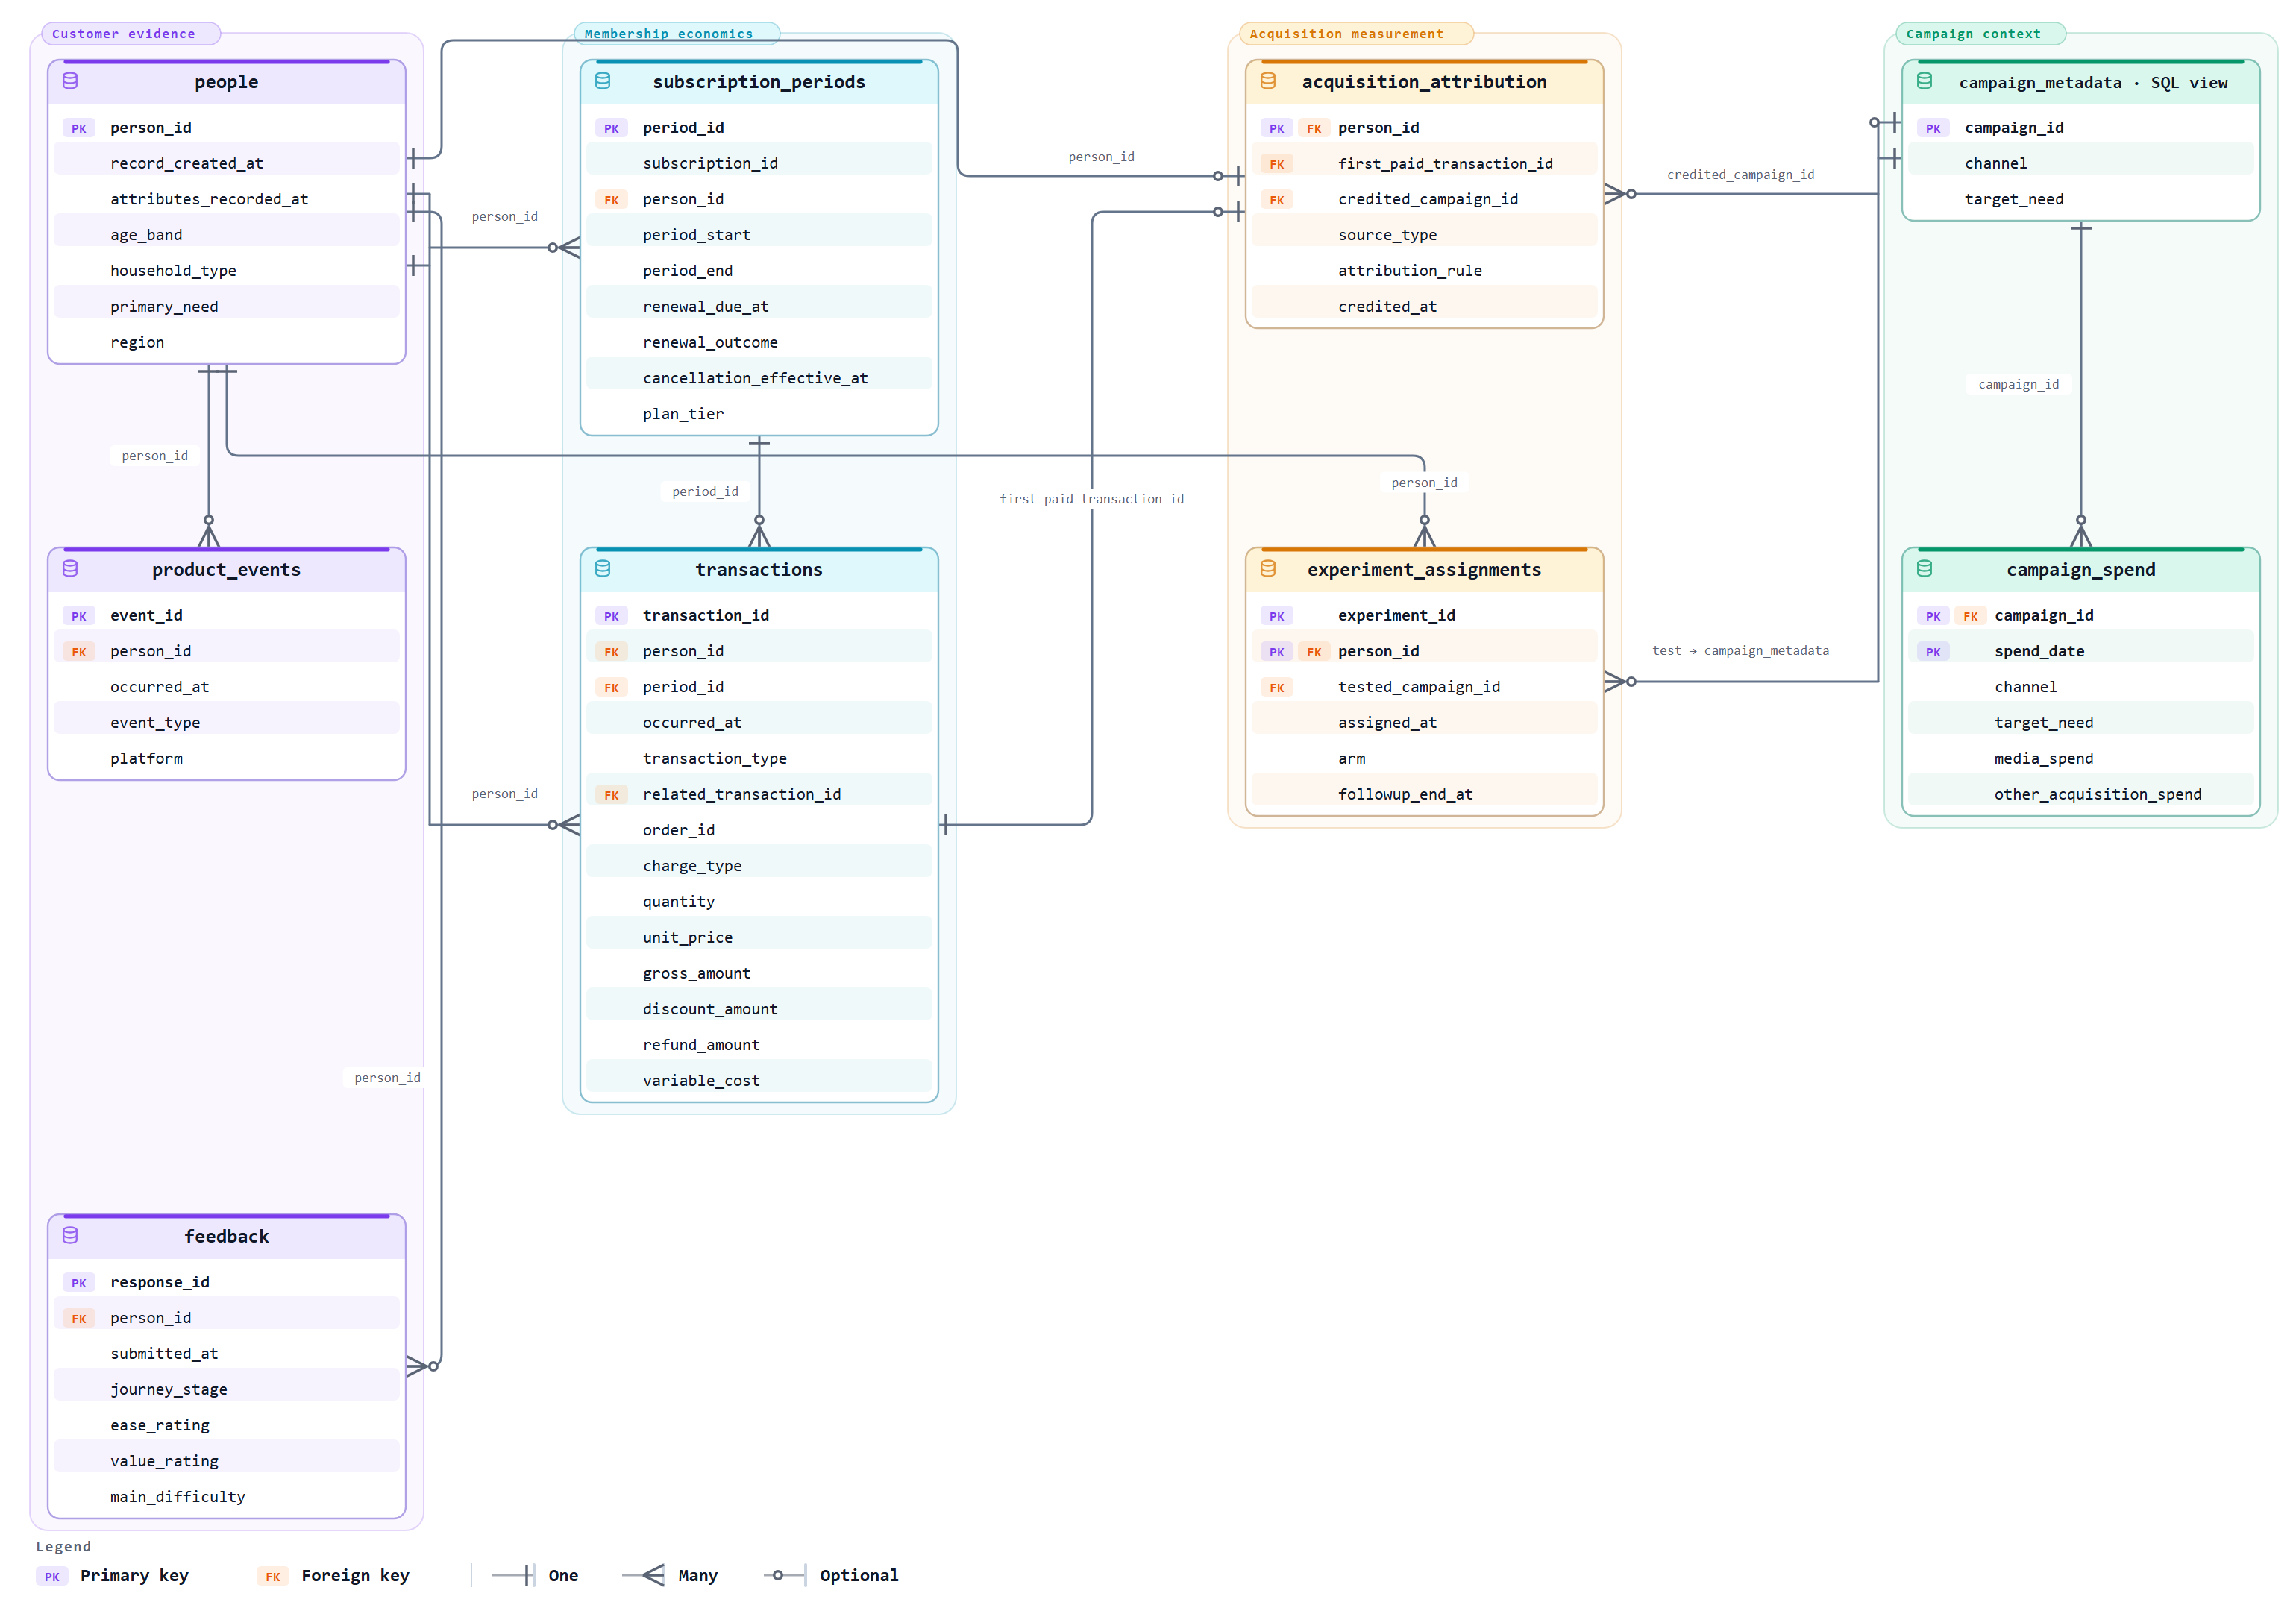
\includegraphics[width=\linewidth,height=8.25in,keepaspectratio]{figures/source-tables-report.png}\end{center}
\Evidence{Native Archify schema; editable SVG/HTML: diagrams/source-tables. Refunds link transactions.related\_transaction\_id to transactions.transaction\_id within the same ledger. Campaign foreign keys target unique campaign\_metadata; campaign\_spend uses campaign\_id + spend\_date. Aggregate to the intended grain before joining one-to-many records.}
\EndSchemaFoldout
\PageTitle{A7 / UNIVERSAL CUSTOMER VIEW}{Classify each source\newline by what it actually measures}{Technical appendix | Identifiers include keys and profile descriptors; engagement records behavior; relationship describes the arrangement; perception records expressed views.}
\DatasetTitle{people.csv}{CRM | One person, including eligible prospects who never purchase.}
{\fontsize{8}{10}\selectfont\begin{tabularx}{\linewidth}{@{}YYYY@{}}\toprule
\textbf{Identifiers} & \textbf{Engagement} & \textbf{Relationship} & \textbf{Perception}\\\midrule
\texttt{person\_\allowbreak{}id}\newline \texttt{age\_\allowbreak{}band}\newline \texttt{household\_\allowbreak{}type}\newline \texttt{region} & \textcolor{BriefMuted}{Not observed} & \texttt{record\_\allowbreak{}created\_\allowbreak{}at}\newline \texttt{attributes\_\allowbreak{}recorded\_\allowbreak{}at} & \texttt{primary\_\allowbreak{}need}\\\bottomrule\end{tabularx}}\par

\DatasetTitle{subscription\_periods.csv}{Renewal system | One scheduled monthly cycle; a paid outcome establishes retained membership for that cycle.}
{\fontsize{8}{10}\selectfont\begin{tabularx}{\linewidth}{@{}YYYY@{}}\toprule
\textbf{Identifiers} & \textbf{Engagement} & \textbf{Relationship} & \textbf{Perception}\\\midrule
\texttt{period\_\allowbreak{}id}\newline \texttt{subscription\_\allowbreak{}id}\newline \texttt{person\_\allowbreak{}id} & \textcolor{BriefMuted}{Not observed} & \texttt{period\_\allowbreak{}start}\newline \texttt{period\_\allowbreak{}end}\newline \texttt{renewal\_\allowbreak{}due\_\allowbreak{}at}\newline \texttt{renewal\_\allowbreak{}outcome}\newline \texttt{cancellation\_\allowbreak{}effective\_\allowbreak{}at}\newline \texttt{plan\_\allowbreak{}tier} & \textcolor{BriefMuted}{Not observed}\\\bottomrule\end{tabularx}}\par

\DatasetTitle{transactions.csv}{Finance | One payment or refund event; each payment is one order and refunds reuse its order ID.}
{\fontsize{8}{10}\selectfont\begin{tabularx}{\linewidth}{@{}YYYY@{}}\toprule
\textbf{Identifiers} & \textbf{Engagement} & \textbf{Relationship} & \textbf{Perception}\\\midrule
\texttt{transaction\_\allowbreak{}id}\newline \texttt{person\_\allowbreak{}id}\newline \texttt{period\_\allowbreak{}id}\newline \texttt{related\_\allowbreak{}transaction\_\allowbreak{}id}\newline \texttt{order\_\allowbreak{}id} & \texttt{occurred\_\allowbreak{}at}\newline \texttt{transaction\_\allowbreak{}type}\newline \texttt{charge\_\allowbreak{}type}\newline \texttt{quantity}\newline \texttt{gross\_\allowbreak{}amount}\newline \texttt{discount\_\allowbreak{}amount}\newline \texttt{refund\_\allowbreak{}amount} & \texttt{unit\_\allowbreak{}price}\newline \texttt{variable\_\allowbreak{}cost} & \textcolor{BriefMuted}{Not observed}\\\bottomrule\end{tabularx}}\par

\DatasetTitle{product\_events.csv}{Product and support | One observed product/support interaction; no event does not mean no subscription.}
{\fontsize{8}{10}\selectfont\begin{tabularx}{\linewidth}{@{}YYYY@{}}\toprule
\textbf{Identifiers} & \textbf{Engagement} & \textbf{Relationship} & \textbf{Perception}\\\midrule
\texttt{event\_\allowbreak{}id}\newline \texttt{person\_\allowbreak{}id} & \texttt{occurred\_\allowbreak{}at}\newline \texttt{event\_\allowbreak{}type}\newline \texttt{platform} & \textcolor{BriefMuted}{Not observed} & \textcolor{BriefMuted}{Not observed}\\\bottomrule\end{tabularx}}\par

\Evidence{Each raw field appears once in its dataset's classification. Source-specific rationale is preserved in \texttt{diagrams/ucv-tables.json}. A category marked not observed is a data gap, not an invitation to infer a missing attitude or relationship.}

\NewPage
\PageTitle{A8 / UNIVERSAL CUSTOMER VIEW}{Keep campaign credit,\newline response and belief distinct}{Technical appendix | Campaign spending and randomized assignment describe different objects from a customer's behavior or survey response.}
\DatasetTitle{feedback.csv}{Customer research | One completed linked survey response; nonresponse is missing, not a zero rating.}
{\fontsize{8}{10}\selectfont\begin{tabularx}{\linewidth}{@{}YYYY@{}}\toprule
\textbf{Identifiers} & \textbf{Engagement} & \textbf{Relationship} & \textbf{Perception}\\\midrule
\texttt{response\_\allowbreak{}id}\newline \texttt{person\_\allowbreak{}id} & \texttt{submitted\_\allowbreak{}at}\newline \texttt{journey\_\allowbreak{}stage} & \textcolor{BriefMuted}{Not observed} & \texttt{ease\_\allowbreak{}rating}\newline \texttt{value\_\allowbreak{}rating}\newline \texttt{main\_\allowbreak{}difficulty}\\\bottomrule\end{tabularx}}\par

\DatasetTitle{campaign\_spend.csv}{Marketing spending | One campaign per spending date; aggregate before joining to customer outcomes.}
{\fontsize{8}{10}\selectfont\begin{tabularx}{\linewidth}{@{}YYYY@{}}\toprule
\textbf{Identifiers} & \textbf{Engagement} & \textbf{Relationship} & \textbf{Perception}\\\midrule
\texttt{campaign\_\allowbreak{}id}\newline \texttt{target\_\allowbreak{}need} & \texttt{spend\_\allowbreak{}date}\newline \texttt{channel}\newline \texttt{media\_\allowbreak{}spend}\newline \texttt{other\_\allowbreak{}acquisition\_\allowbreak{}spend} & \textcolor{BriefMuted}{Not observed} & \textcolor{BriefMuted}{Not observed}\\\bottomrule\end{tabularx}}\par
\Evidence{Campaign-level operational support for acquisition economics, not individual engagement.}

\DatasetTitle{acquisition\_attribution.csv}{Marketing attribution | One acquired person and the recorded credit for the first successful payment.}
{\fontsize{8}{10}\selectfont\begin{tabularx}{\linewidth}{@{}YYYY@{}}\toprule
\textbf{Identifiers} & \textbf{Engagement} & \textbf{Relationship} & \textbf{Perception}\\\midrule
\texttt{person\_\allowbreak{}id}\newline \texttt{first\_\allowbreak{}paid\_\allowbreak{}transaction\_\allowbreak{}id}\newline \texttt{credited\_\allowbreak{}campaign\_\allowbreak{}id} & \texttt{source\_\allowbreak{}type}\newline \texttt{credited\_\allowbreak{}at}\newline \texttt{attribution\_\allowbreak{}rule} & \textcolor{BriefMuted}{Not observed} & \textcolor{BriefMuted}{Not observed}\\\bottomrule\end{tabularx}}\par
\Evidence{Measurement metadata for engagement credit, not a customer action itself.}

\DatasetTitle{experiment\_assignments.csv}{Experiment platform | One eligible person per randomized experiment, including all nonbuyers.}
{\fontsize{8}{10}\selectfont\begin{tabularx}{\linewidth}{@{}YYYY@{}}\toprule
\textbf{Identifiers} & \textbf{Engagement} & \textbf{Relationship} & \textbf{Perception}\\\midrule
\texttt{experiment\_\allowbreak{}id}\newline \texttt{person\_\allowbreak{}id}\newline \texttt{tested\_\allowbreak{}campaign\_\allowbreak{}id} & \textcolor{BriefMuted}{Not observed} & \texttt{assigned\_\allowbreak{}at}\newline \texttt{arm}\newline \texttt{followup\_\allowbreak{}end\_\allowbreak{}at} & \textcolor{BriefMuted}{Not observed}\\\bottomrule\end{tabularx}}\par
\Evidence{Experimental relationship/design metadata; assignment is not observed exposure or purchase.}

\Section{Sources and model adaptations}
Juan Orduz, Revenue Retention and Customer Lifetime Value with NumPyro; Peter Fader and Bruce Hardie, contractual-customer retention and shifted-Beta-Geometric models; Gil Bouhnick, Cohort Analysis. Exact links, adaptation boundaries and licensing are retained in the repository source documentation. Archify is pinned and redistributed with its license notices.
\Evidence{Retention extends Fader-Hardie sBG with mean/concentration parameterization, logit/log covariate links, a non-centered cohort effect on mean churn, grouped conditional Binomial renewal likelihood and NUTS estimation. Revenue adapts Orduz's Gamma structure but uses observed active counts in fitting, an additional per-member shape multiplier, a mean link without an age-by-cohort interaction, need/channel covariates and \$100 scaling. Conditional on observed activity, the revenue and retention likelihoods have independent parameter blocks. The separate Orduz-inspired 4-hidden-unit Bayesian neural network is a retention comparison only; its cumulative-count likelihood is changed to conditional renewal trials.}
\Evidence{All graphics in this report are generated from this repository's original synthetic records or original diagram specifications. The public sources motivate analytical ideas; their screenshots and private course materials are not redistributed.}
\end{document}